\documentclass[10pt,a4paper]{article}
\usepackage[utf8]{inputenc}
\usepackage[spanish]{babel}
\usepackage{amsmath}
\usepackage{amsfonts}
\usepackage{amssymb}
\usepackage{graphicx}
\usepackage{array}
\author{Erick de Jesus Hernández Cerecedo}
\title{Resumen del texto Metodolog\'ias \'Agiles de Desarrollo Software}
\begin{document}
\maketitle

\section{Introducci\'on}
El siguiente documento contiene un resumen del texto ``Metodolog\'ias  \'Agiles de Desarrollo de Software Aplicadas a la Gesti\'on de Proyectos Empresariales'' (L\'opez G, 2015) de done se rescatan los temas m\'as destacados.

\section{Gesti\'on de Proyectos Inform\'aticos Empresariales}
Un Proyecto informatico es un sistema de cursos de acciones simultaneas  y/o secuenciales que involucran personas, equipamientos de hardware, software y comunicaciones, enfocadas en obtener uno o m\'as resultados deseables sobre un sistema de informacion.
Las organizaciones o empresas emplean este tipo de proyectos con el fin de generar diferenciadores respecto a sus competidores y la forma m\'as eficiente es implementar un sistema de gesti\'on de proyectos.

\begin{figure}[h]
	\centering
	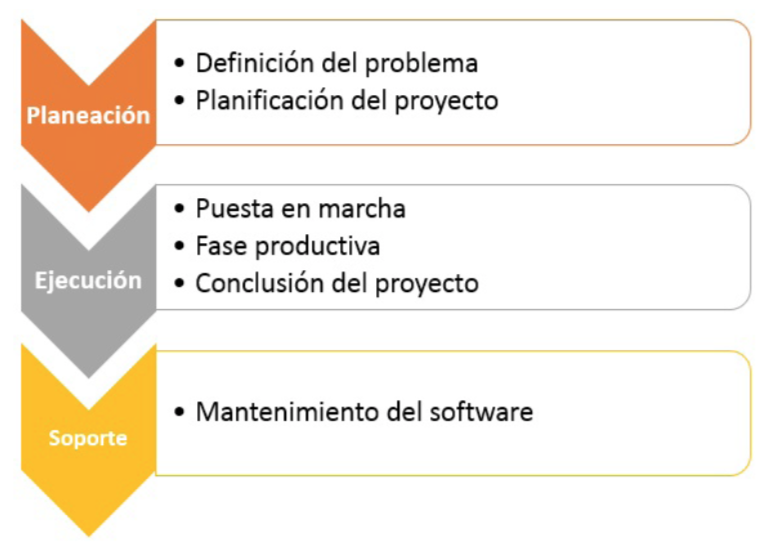
\includegraphics[scale=0.6]{fases.png}
	\caption{Fases Principales de un Proyecto de Desarrollo de Software}
\end{figure}

Clasificaci\'on de los proyectos inform\'aticos:
\begin{itemize}
	\item Software
	\item Hardware
	\item Comunicaciones y Redes
	\item Instalaciones de Hardware
	\item Auditoria, etc.
\end{itemize}


\section{Fases Principales de un Proyecto de Desarrollo de Software}
\begin{enumerate}
	\renewcommand{\theenumi}{\Alph{enumi}}
	\item Planeaci\'on
		\begin{list}{}{}
			\item En esta fase se plantean los objetivos del proyecto, considerando las tres diemensiones sobre las que se apoya todo proyecto.
			\begin{itemize}
				\item Calidad
				\item Costo
				\item Tiempo de curaci\'on
			\end{itemize}
		\end{list}	
	\item Ejecuci\'on
		\begin{list}{}{}
			\item En esta fase se pone en pr\'actica lo planeado en la fase anterior, es decir una mala planeaci\'on traer\'a resultados negativos a la ejecuci\'on de u proyecto.
		\end{list}
	
	\item Soporte
		\begin{list}{}{}
			\item Tambien llamada fase mantenimiento viene despues de la implementaci\'on, consiste en mantener al softwae operando en \'optimas condiciones y verificando que no existan fallas. 
		\end{list}
	
\end{enumerate}

\section{Metodolog\'ias \'Agiles de Desarrollo}
Son una iniciativa de un conjunto de expertos en el \'area de desarrollo de software con el fin de optimizar el proceso de creaci\'on del mismo, el punto de partida fue el manifiesto ``\'Agil''. \\ \par

\textbf{Manifiesto \'Agil}\\ \par
Este documento engloba principios y valores que hacen diferente un proyecto de software \'agil de uno tradicional, esta regida por doce principios que ayudan a que el proceso se vuelva menos complejo y responda de manera oportuna a los cambios que surjan, siempre contando con el punto de vista del cliente. \par

\begin{figure}[h]
	\centering
	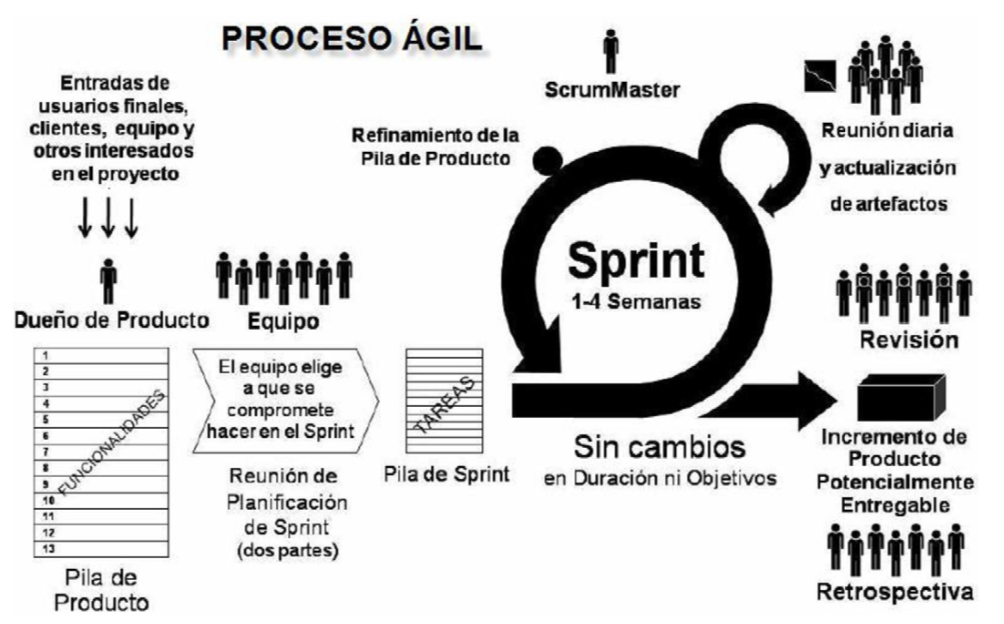
\includegraphics[scale=0.6]{agil.png}
	\caption{Proceso \'Agil de Desarrollo de Software}
\end{figure}

Seg\'un el manifiesto se valora:
\begin{itemize}
	\item Al individuo y la interacciones del equipo de desarrollo sobre el proceso y la herramientas.
	\item Desarrollar software que funcione m\'as rapido que la documentaci\'on del mismo.
	\item La colaboraci\'on con el cliente m\'as que la negociaci\'on de su contrato.
	\item Responde a los cambios m\'as que seguir con el plan establecido.
\end{itemize}

\textbf{Principales Metodologias \'Agiles}
\begin{enumerate}
	\renewcommand{\theenumi}{\Alph{enumi}}
	\item Scrum
		\begin{list}{}{}
			\item Scrum se basa en la teor\'ia de control de procesos emp\'irica, que asegura que el conocimiento procede de la experiencia y de tomar decisiones bas\'andese en lo que se conoce. Existen tres pilares fundamentales que soportan el control del proceso emp\'irico los cuales son:
				\begin{itemize}
					\item Transparencia
					\item Inspecci\'on
					\item Adaptaci\'on
				\end{itemize}
			\item La metodolog\'ia \textit{Scrum} describe cuatro eventos importantes que componen cada una de las entregas:
				\begin{itemize}
					\item\textit{Reunion de planificaci\'on del sprint (Sprint Planing Meeting)}
					\item \textit{Scrum Diario (Daily Scrum)}
					\item \textit{Revision del Sprint (Sprint Review)}
					\item\textit{Retrospectiva del Sprint (Sprint Retrospective)}
				\end{itemize}	
			\item Scrum se centra en la divisi\'on del trabajo complete (Product Backlog) en distintos apartados o bloques que pueden ser abordados en periodos cortos de tiempo (1 -4 semanas), los cuales son denominados Sprint.					
		\end{list}	
		\begin{figure}[h]
			\centering
			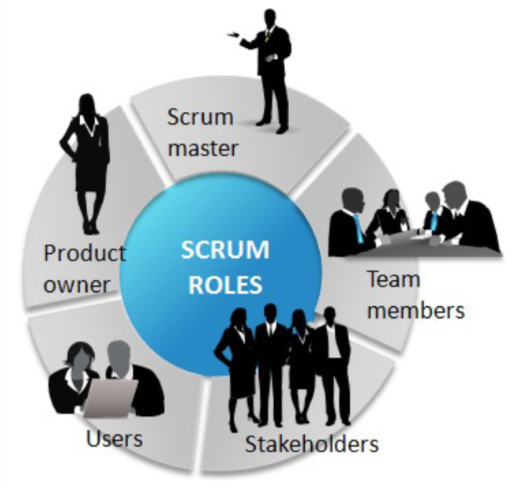
\includegraphics[scale=0.6]{scrum.png}
			\caption{Equipo de Trabajo de la Metodolog\'ia Srum}
		\end{figure}
	
	\item Extreme Programming (XP)
		\begin{list}{}{}
			\item La programaci\'on extrema es una metodolog\'ia que se basa en una seria de reglas y principios que se han utilizado a lo largo de toda la historia del desarrollo del software, en el que cada una de ellas se aplican conjuntamente, se le \'enfasis a las tareas que agreguen valor de manera que creen un proceso \'agil.
			\item Se engloba en 12 principios b\'asicos los cuales se agrupan en cuatro categor\'ias grandes:
				\begin{itemize}
					\item \textit{Retroalimentaci\'on a Escala Fina}, en esta fase se encuentran diversos principios, realizaci\'on de pruebas, proceso de planificaci\'on en parejas.
					\item \textit{Proceso Continuo en lugar de por lotes}, permite la integraici\'on continua, refactorizaci\'on y entregas peque\~nas.
					\item \textit{Entendimiento compartido}, en esta categor\'ia se definen criterios como el de crear un diseño f\'acil, las tarjetas CRC y la creaci\'on de la met\'afora del sistema o historia completa.
					\item \textit{Bienestar del programador}, se rige por la filosof\'ia que un programador cansado, exhausto crea c\'odigo de mala calidad, por eso se recomienda que los desarrolladores tengan 40 horas de trabajo a la semana y muy pocas horas de trabajo extra.
				\end{itemize}						
			
		\end{list}	
		\begin{figure}[h]
			\centering
			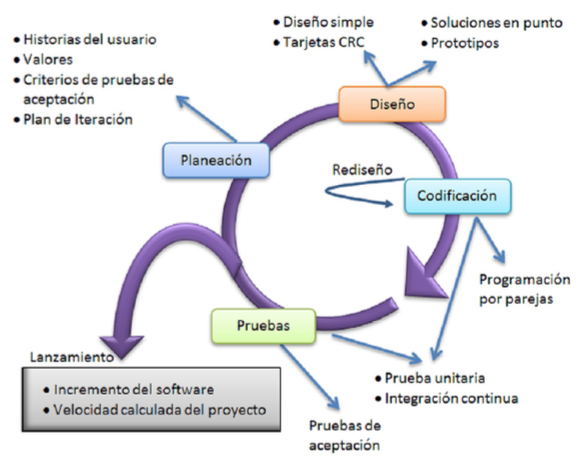
\includegraphics[scale=0.6]{extreme.png}
			\caption{Macro de trabajo de la metodolog\'ia XP.}
		\end{figure}	
		
	\item Crystal Clear
		\begin{list}{}{}
			\item Crystal es una metodolog\'ia en la cual se establecen c\'odigos de color como parte de la definici\'on de la complejidad de la misma, si es m\'as oscuro entonces el m\'etodo es m\'as pesado, todo esto en funci\'on de su criticidad y tama\~no.
			\item Lista de riesgos potenciales:
				\begin{itemize}
					\item \textbf{C:} P\'erdida de confort debido a un fallo del sistema.
					\item \textbf{D:} P\'erdida de dinero discrecional (nuestro dinero)
					\item \textbf{E:} P\'erdida de dinero esencial (Este es el dinero del cual no se puede disponer).
					\item \textbf{C:} P\'erdida de vidas por el fallo del sistema. 
				\end{itemize}							
			\item Los n\'umero indican la cantidad de personas que son coordinadas en el proyecto, de acuerdo a lo siguiente:
				\begin{itemize}
					\item Clear es para equipos de 8 perosnas o menos.
					\item Amarillo para equipos de 10 - 20 personas.
					\item Naranja para equipos de 20 - 50 perosnas.
					\item Rojo es para equipos  de 50 - 100 y as\'i sucesivamente pasando por el marr\'on y violeta.
				\end{itemize}						
		\end{list}
		
		\begin{figure}[h]
			\centering
				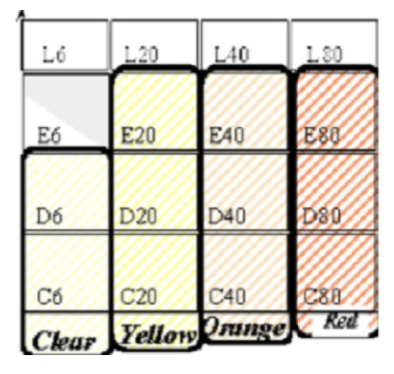
\includegraphics[scale=0.6]{crystal.png}
			\caption{Criticidad de la metodolog\'ia Crystal.}
		\end{figure}	

\end{enumerate}


\section{Plataformas y Arquitecturas}
De la misma forma en que se cuenta con diversas metodolog\'ias de \'agiles de desarrollo de software, se cuenta con plataformas en las que se pueden ejecutar, algunas de estas herramientas traen una versi\'on de prueba y otra de paga ademas de herramientas en la nube.

\begin{list}{}{}
	\item \textit{OpenProject}
	\item IceScrum
	\item TeamWork
	\item X Planner
	\item Agile Mantis
\end{list}

\section{Metodolog\'ias Tradicionales VRS \'Agiles}
La incorporaci\'on de nuevas tecnologias y formas de llevar a cabo el proceso de desarrollo de software ha venido revolucionando de tal manera que se han dejado los procesos largos y documentaci\'on exhaustiva, por m\'etodos m\'as enfocados en el cliente y en el equipo de desarrollo.

\begin{table}[h]
	\begin{center}
		\begin{tabular}{ | c | m{5cm} | m{5cm} | }
			\hline Aspectos & \'Agil & Dirigido por Modelos \\
			\hline Personas & Alta prioridad; se facilita relaci\'on cliente desarrollador & No prioritaio: El modelo del espacio del problema es la base de la discusi\'on entre cliente-desarrollador \\
			\hline Proceso & Prioridad media; Incremental y evolutivo & Tiende al proceso en cascada; poco incremental \\
			\hline Tecnolog\'ia & Baja prioridad: Solo cobra importancia al final & Es relevante; se usa para la generaci\'on del software (usando un PSM)\\
			\hline Modelos & Artefacto secundario; Se producen cuando es absolutamente necesario & Artefacto prioritario; Fuente de la implementaci\'on\\
			\hline Software & Artefacto prioritario; Es la \'unica medida de progreso & Artefacto secundario; depende del espacio de la soluci\'on \\ \hline
		\end{tabular}	
		\caption{Tabla comparativa M\'etodo \'Agil vs Tradicional}		
	\end{center}
\end{table}

\end{document}